\section{Additional examples for a Gaussian hierarchical inference}
\label{app: additional gaussians}

\subsection{Parameter Estimation uncertainty only}
\label{app: gaussian pe uncertainty only}

Here we show additional examples from Sec.~\ref{subsec: mc example without selection effects} of the Gaussian hierarchical inference with $\Nobs = 1000$ and $\Nobs = 5000$. Notice the error statistic scalings are roughly matched by the analytic predictions in Table~\ref{tab: scaling}. Restricting our attention to $\NPE = 1000$, in Figs.~\ref{fig: nobs 100 gaussian example},~\ref{fig: nobs 1000 gaussian example} and~\ref{fig: nobs 5000 gaussian example} we have $\Nobs=100$, $1000$, and $5000$ and $\hat{\Pi}[\hat{p}]\sim 10^{-2}$: roughly constant in $\Nobs$. 
The accuracy statistics scale roughly linearly: $\hat{A}[\hat{p}]\sim 5\times10^{-4}, 5\times10^{-3}, 0.02$ bits. For a more quantitative scaling analogous to our precision statistic scaling, see Fig. 2 in \citet{Essick:2022ojx}.

\begin{figure}[h!]
    \centering
    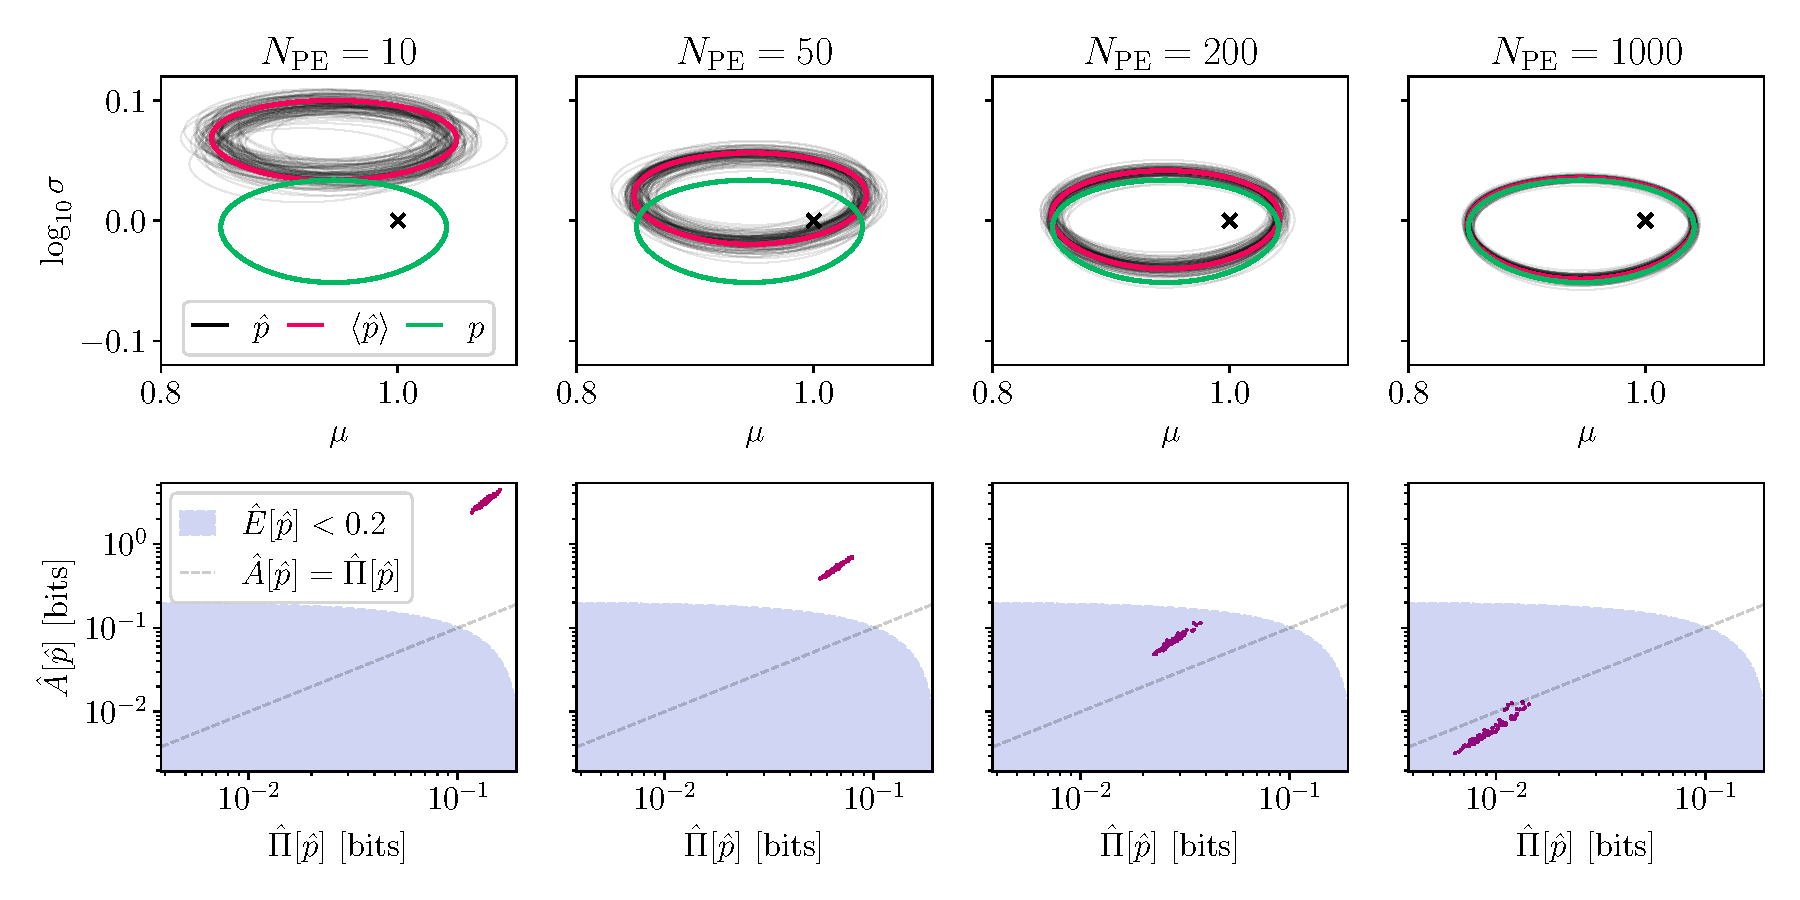
\includegraphics[width=\linewidth]{plots/gaus_hierarchical/pe_uncertainty_only/N1000_4pes_scatter.pdf}
    \caption{Same as Fig.~\ref{fig: nobs 100 gaussian example}, but with 1000 observations. Note the zoomed in x- and y-axes relative to Fig.~\ref{fig: nobs 100 gaussian example}. }
    \label{fig: nobs 1000 gaussian example}
\end{figure}

\begin{figure}[h!]
    \centering
    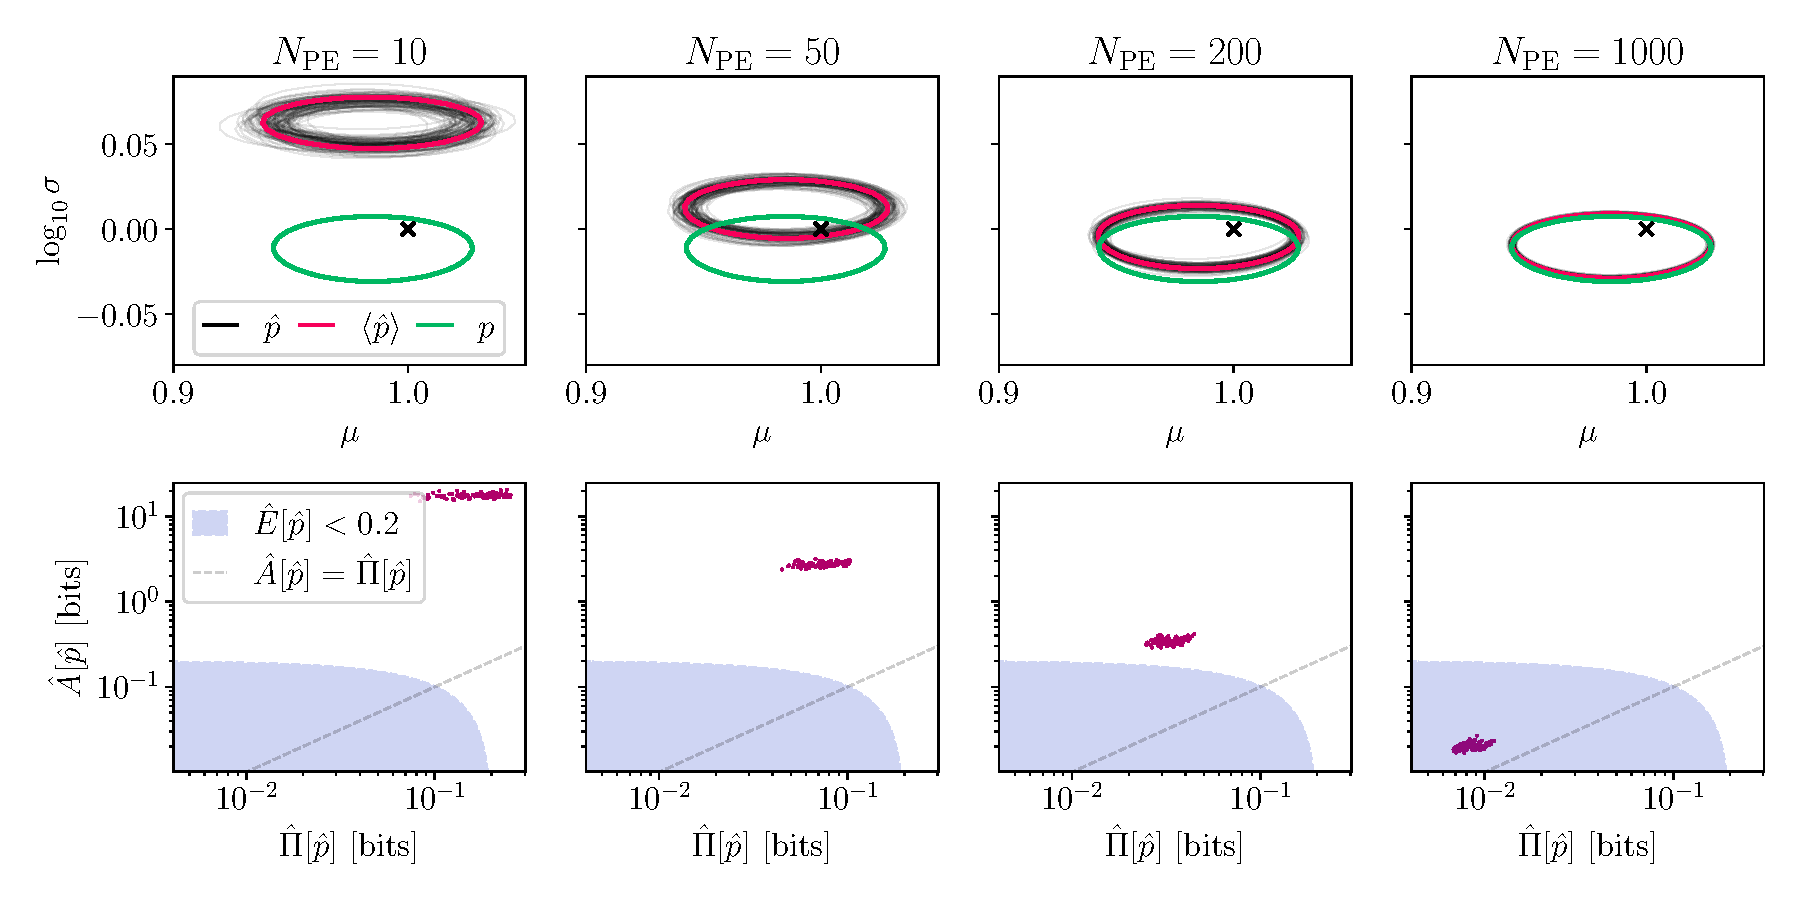
\includegraphics[width=\linewidth]{plots/gaus_hierarchical/pe_uncertainty_only/N5000_4pes_scatter.pdf}
    \caption{Same as Fig.~\ref{fig: nobs 100 gaussian example}, but with 5000 observations. Note the zoomed in x- and y-axes relative to Fig.~\ref{fig: nobs 100 gaussian example}. }
    \label{fig: nobs 5000 gaussian example}
\end{figure}

We also show examples where the noise is larger than the scale of the population: each single event posterior is larger than the width of the population. The hyperposteriors are correspondingly broader, and we see that we require much larger $\NPE$ in order to obtain a similar level of precision and accuracy. We include this to emphasize that the size of $\NPE$ necessary can vary significantly over different applications.

\begin{figure}[h!]
    \centering
    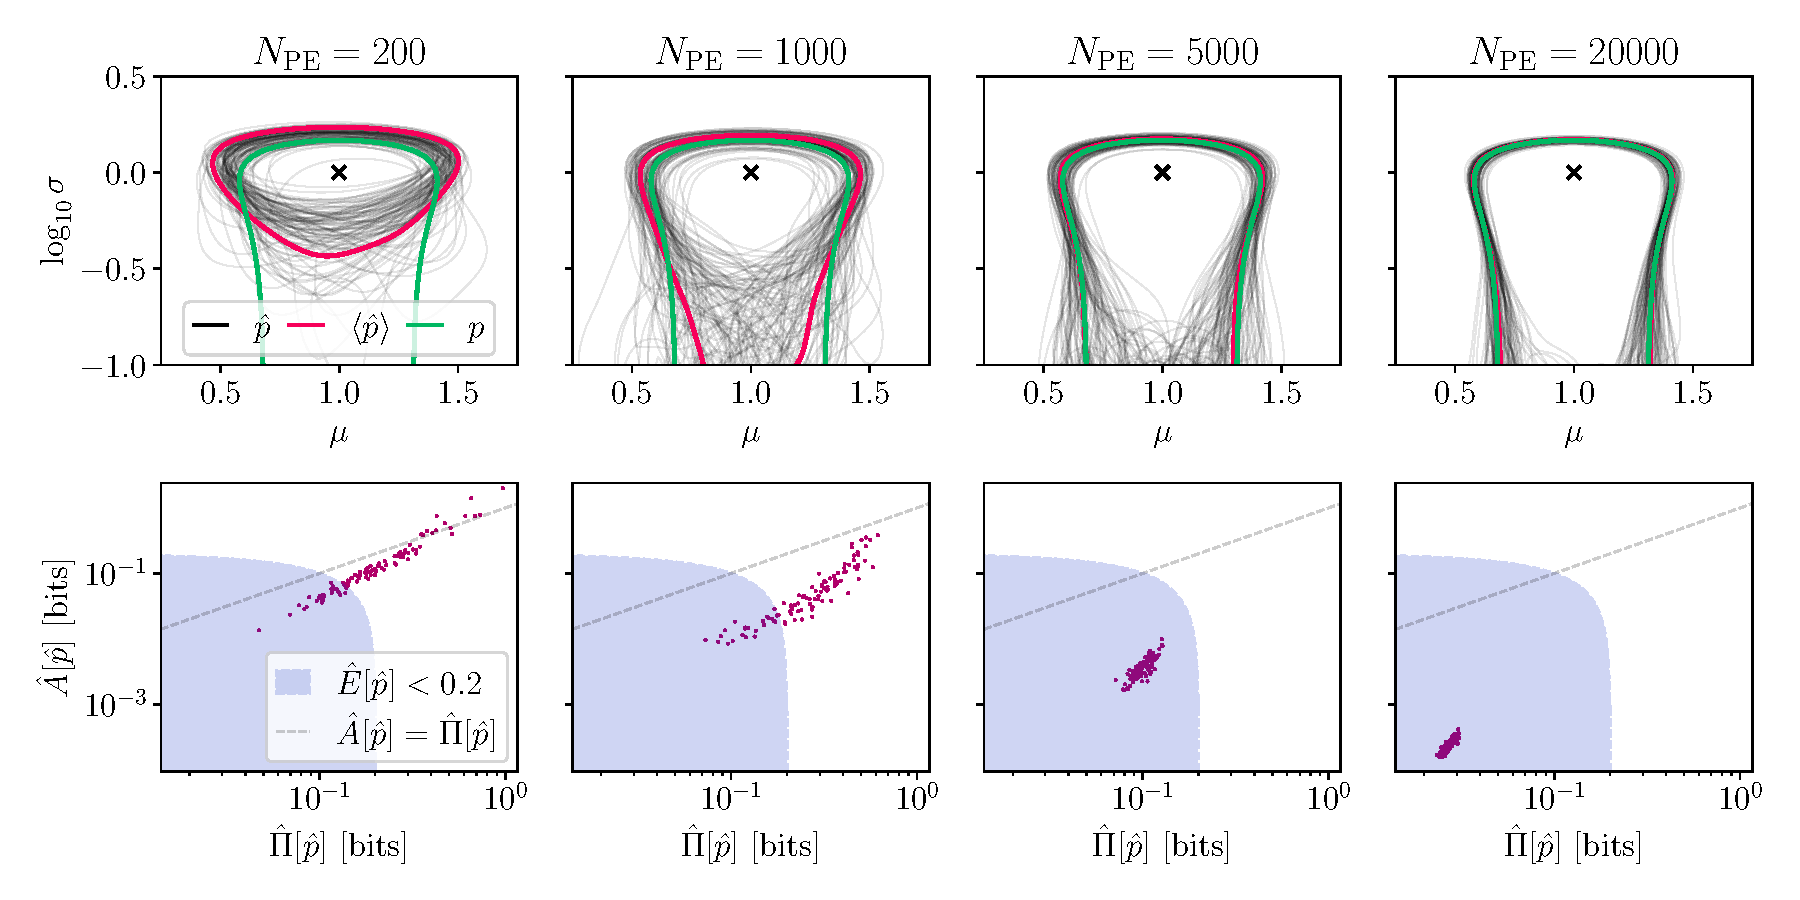
\includegraphics[width=\linewidth]{plots/gaus_hierarchical/pe_uncertainty_only/large_noise_N100_4pes_scatter.pdf}
    \caption{Same as Fig.~\ref{fig: nobs 100 gaussian example}, but with $\Nobs=100$ observations with larger noise $\sigma_n=2$ than the scale of the population $\sigma=1$. }
    \label{fig: nobs 100 larger noise}
\end{figure}

\begin{figure}[h!]
    \centering
    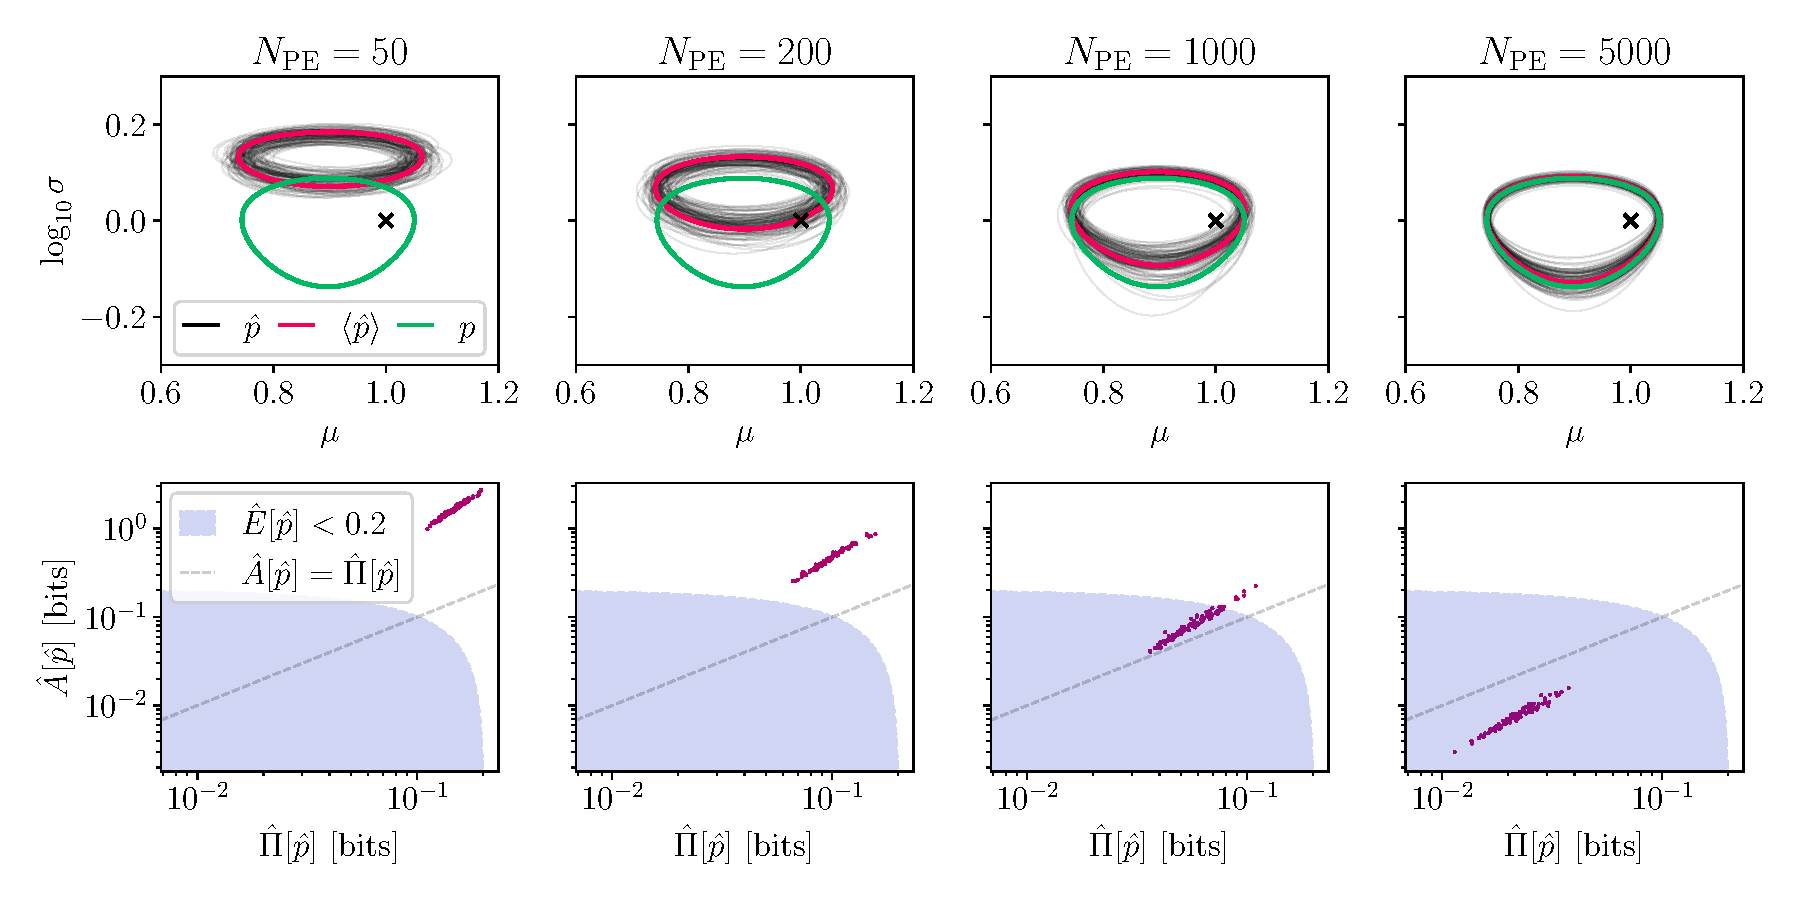
\includegraphics[width=\linewidth]{plots/gaus_hierarchical/pe_uncertainty_only/large_noise_N1000_4pes_scatter.pdf}
    \caption{Same as Fig.~\ref{fig: nobs 100 gaussian example}, but with $\Nobs=1000$ observations with larger noise $\sigma_n=2$ than the scale of the population $\sigma=1$. }
    \label{fig: nobs 1000 larger noise}
\end{figure}

\begin{figure}[h!]
    \centering
    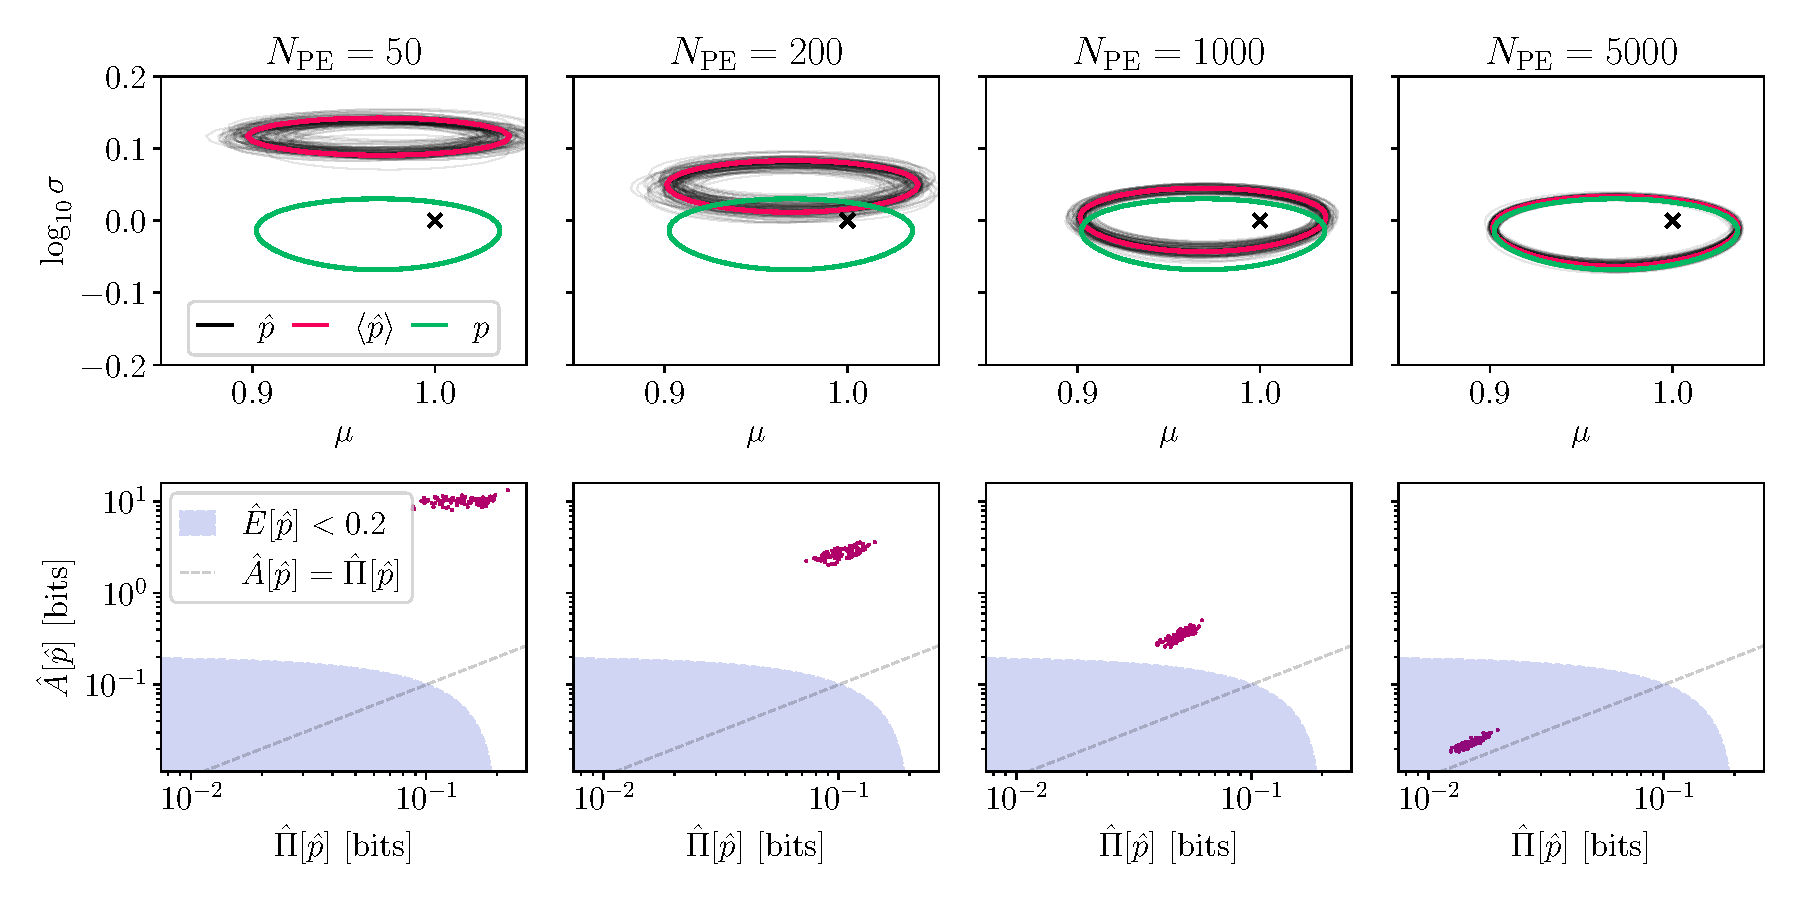
\includegraphics[width=\linewidth]{plots/gaus_hierarchical/pe_uncertainty_only/large_noise_N5000_4pes_scatter.pdf}
    \caption{Same as Fig.~\ref{fig: nobs 100 gaussian example}, but with $\Nobs=5000$ observations with larger noise $\sigma_n=2$ than the scale of the population $\sigma=1$. }
    \label{fig: nobs 5000 larger noise}
\end{figure}

\clearpage
% \newpage

\subsection{Selection effects estimation uncertainty only}
\label{app: gaussian vt uncertainty only}

We include some additional examples to Sec.~\ref{subsec: mc example with selection effects} where we vary the number of injections $\Ninj$ and the strength of the selection criterion. Some of the posterior estimators shown here are limited by the resolution on the underlying grid of $\sigma$ and $\mu$. 

Note that the scaling is roughly similar to the scaling arguments shown in Table~\ref{tab: scaling}. Restricting our attention to the case with selection $d=\theta+n>1$ and $\Ninj = 10^6$, in Figs.~\ref{fig: nobs 100 corrected vt 1 gaussian example},~\ref{fig: nobs 1000 corrected vt 1 gaussian example}, and~\ref{fig: nobs 5000 corrected vt 1 gaussian example} we have $\Nobs=100$, $1000$, and $5000$ and $\hat{\Pi}[\hat{p}]\sim 0.005, 0.03, 0.1$ bits: scaling roughly linearly in $\Nobs$. Note the posteriors are far from Gaussian, for $\Nobs = 100$, and so the scaling does not yet kick in.
For a more quantitative scaling analogous to our precision statistic scaling, see Fig. 3 in \citet{Essick:2022ojx}.

As for the scaling of the accuracy statistic, for $\Ninj = 10^6$ in Figs.~\ref{fig: nobs 100 corrected vt 1 gaussian example},~\ref{fig: nobs 1000 corrected vt 1 gaussian example}, and~\ref{fig: nobs 5000 corrected vt 1 gaussian example} we have $\Nobs=100$, $1000$, and $5000$ and $\hat{A}[\hat{p}]\sim 10^{-6}, 10^{-3}, 0.1$ bits, roughly consistent with the $\Nobs^3$ scaling predicted in Table~\ref{tab: scaling}.

\begin{figure}[h!]
    \centering
    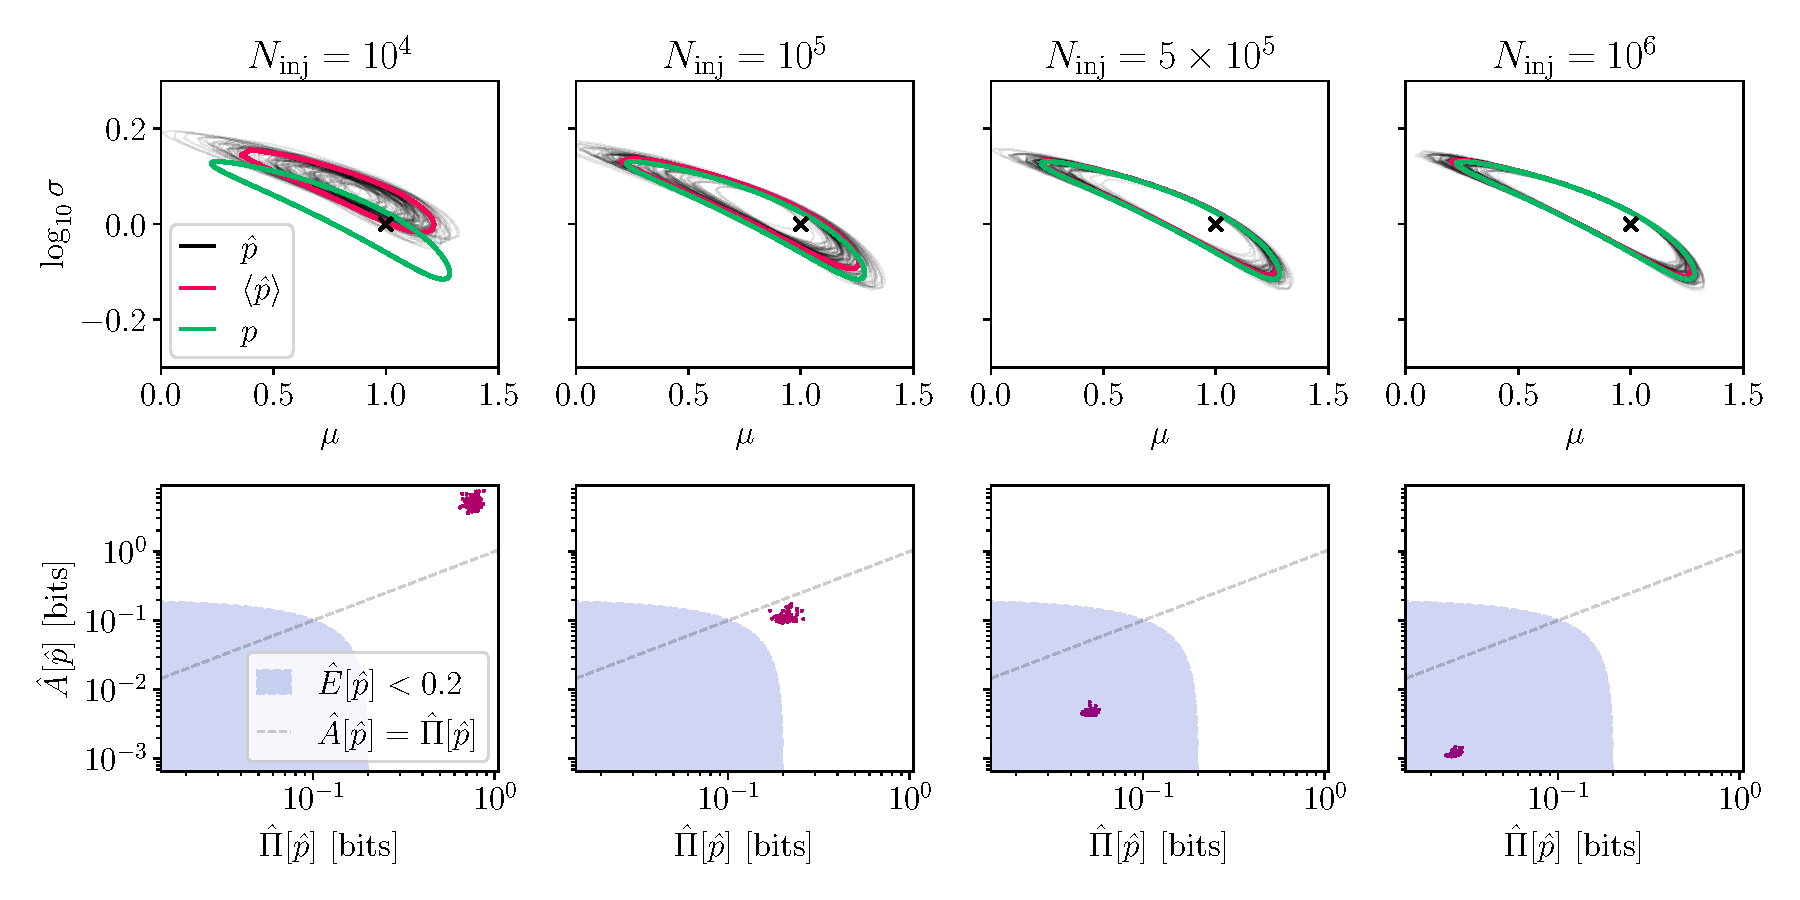
\includegraphics[width=\linewidth]{plots/gaus_hierarchical/selection_effects/selection_1_N1000_4vts_scatter.pdf}
    \caption{Same as Fig.~\ref{fig: nobs 100 corrected vt 1 gaussian example}, with $\Nobs=1000$ observations and the selection given by $d=\theta+n > 1$ and using the corrected likelihood estimator of Eq.~\ref{eq: unbiased likelihood estimator}.}
    \label{fig: nobs 1000 corrected vt 1 gaussian example}
\end{figure}

\begin{figure}[h!]
    \centering
    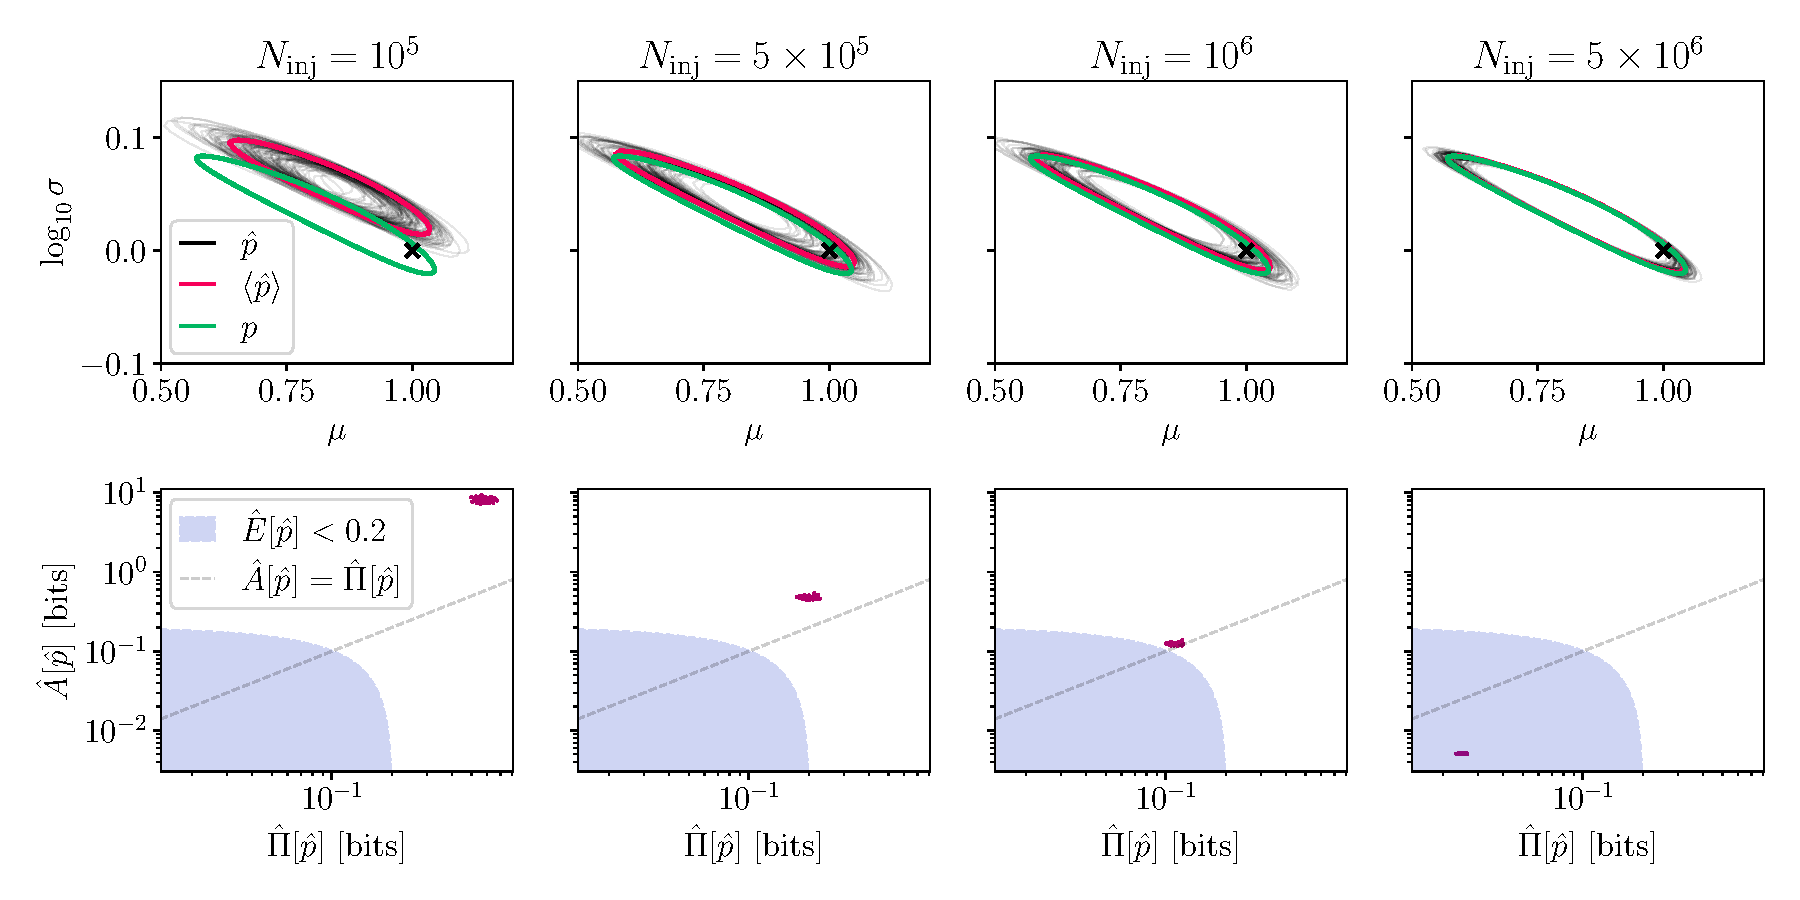
\includegraphics[width=\linewidth]{plots/gaus_hierarchical/selection_effects/selection_1_N5000_4vts_scatter.pdf}
    \caption{Same as Fig.~\ref{fig: nobs 100 corrected  vt 1 gaussian example}, with $\Nobs=5000$ observations and the selection given by $d=\theta+n > 1$ and using the corrected likelihood estimator of Eq.~\ref{eq: unbiased likelihood estimator}.}
    \label{fig: nobs 5000 corrected vt 1 gaussian example}
\end{figure}

When the selection criterion is changed, the shapes and uncertainties in the hierarchical posterior become significantly different. We consider additional inferences where selection is given by $d = \theta+ n > 3$. For the same number of observations $\Nobs$ and injections $\Ninj$, the error statistics in the inference with a stricter selection criterion are much higher.

\begin{figure}[h!]
    \centering
    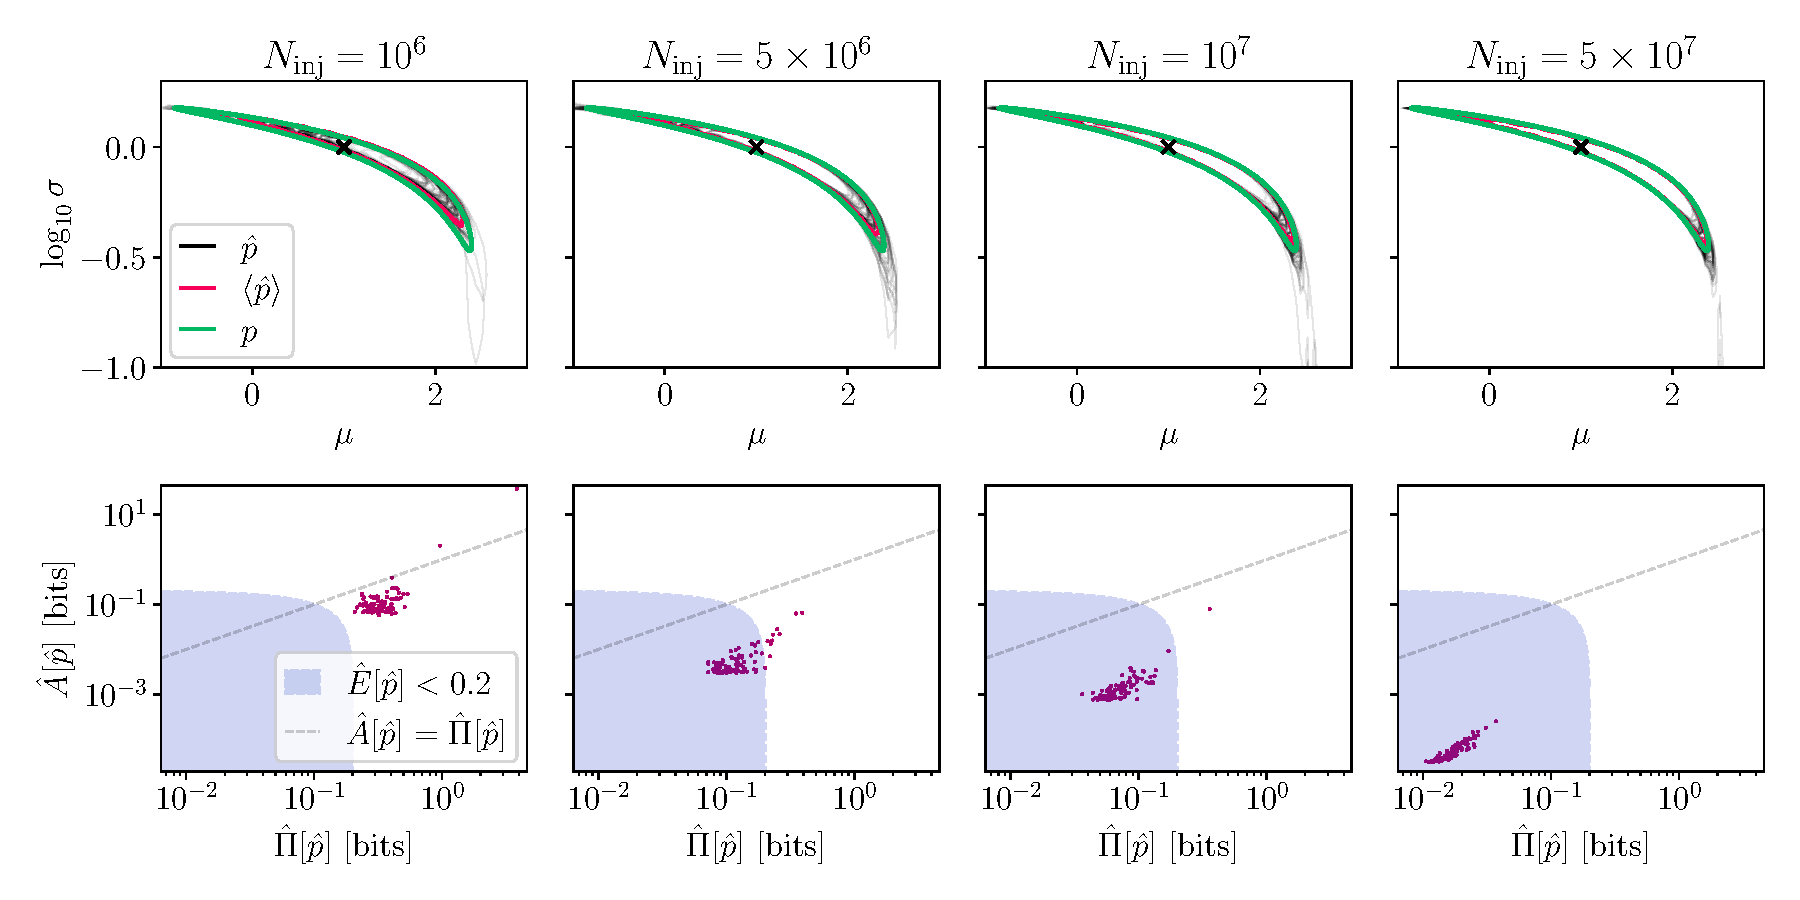
\includegraphics[width=\linewidth]{plots/gaus_hierarchical/selection_effects/selection_3_N1000_4vts_scatter.pdf}
    \caption{Same as Fig.~\ref{fig: nobs 100 corrected vt 1 gaussian example}, with $\Nobs=1000$ observations and the selection given by $d=\theta+n > 3$ and using the corrected likelihood estimator of Eq.~\ref{eq: unbiased likelihood estimator}.}
    \label{fig: nobs 1000 vt 3 gaussian example}
\end{figure}

\begin{figure}[h!]
    \centering
    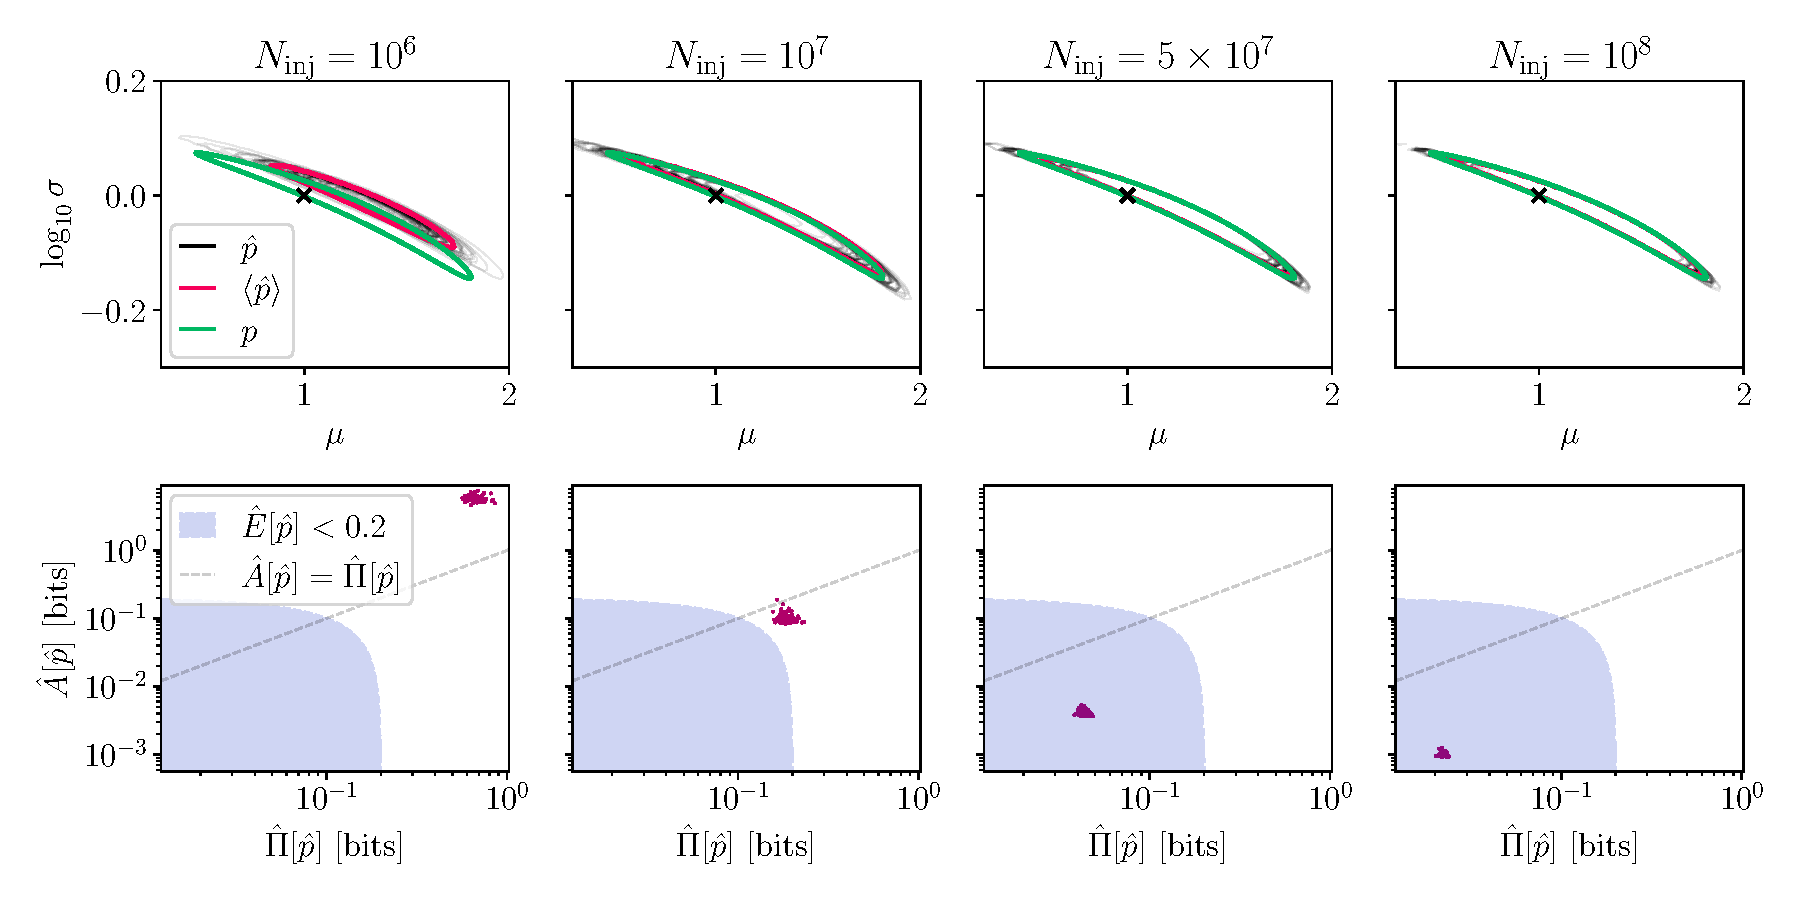
\includegraphics[width=\linewidth]{plots/gaus_hierarchical/selection_effects/selection_3_N5000_4vts_scatter.pdf}
    \caption{Same as Fig.~\ref{fig: nobs 100 corrected vt 1 gaussian example}, with $\Nobs=5000$ observations and the selection given by $d=\theta+n > 3$ and using the corrected likelihood estimator of Eq.~\ref{eq: unbiased likelihood estimator}.}
    \label{fig: nobs 5000 vt 3 gaussian example}
\end{figure}

\clearpage

\section{Examples with posterior correction}
\label{app: examples of posterior correction}

We show some examples of \textit{explicitly} correcting the posterior estimators using the general expression (Eq.~\ref{eq: modifying term}) derived in Appendix~\ref{app: correction in general}. We use the same Gaussian hierarchical inference framework described in Sec.~\ref{sec: mc gaussian example}. 
Instead of estimating the accuracy statistic $\hat{A}$ with Eq.~\ref{eq: accuracy statistic}, however, we calculate the bias correction with the modifying term
\beq
m(\Lambda) = 
\begin{cases}
\exp\left[-\dfrac{1}{2}\dfrac{\Nobs(\Nobs+1)\hat{\sigma}^2_{\xi}(\Lambda)}{\hat{\xi}(\Lambda)^2} + \dfrac{1}{N_{\rm samp}}\displaystyle\sum_{m=1}^{N_{\rm samp}} \hat{C}_{\ln \mathcal{L}}(\Lambda, \Lambda_m)\right] & \begin{tabular}{@{}l@{}}  \text{if using uncorrected} \\ \text{likelihood (Eq.~\ref{eq: estimated hierarchical likelihood})}\end{tabular} \\ 
\exp\left[\dfrac{1}{N_{\rm samp}}\displaystyle\sum_{m=1}^{N_{\rm samp}} \hat{C}_{\ln \mathcal{L}}(\Lambda, \Lambda_m)\right]  & \begin{tabular}{@{}l@{}} \text{if using corrected} \\ \text{likelihood (Eq.~\ref{eq: unbiased likelihood estimator}).}\end{tabular}
\end{cases}
\label{eq: bias correction term}
\eeq
where $\hat{C}_{\ln \mathcal{L}}$ is defined in Eq.~\ref{eq: population covariance with selection}, and 
\beq
\hat{p}_C(\Lambda) \propto \hat{p}(\Lambda)m(\Lambda)
\label{eq: practical posterior correction}
\eeq
is the corrected posterior estimator.

We show an example comparing the uncorrected posterior estimators with the corrected posterior estimator when only parameter estimation uncertainty is considered, as Sec.~\ref{subsec: mc example without selection effects}. We show the example in Fig.~\ref{fig: posterior comparisons nobs 5000} where $\Nobs = 5000$ (where we know from Table~\ref{tab: scaling} that the bias will contribute strongly for small $\NPE$).

\begin{figure}
    \centering
    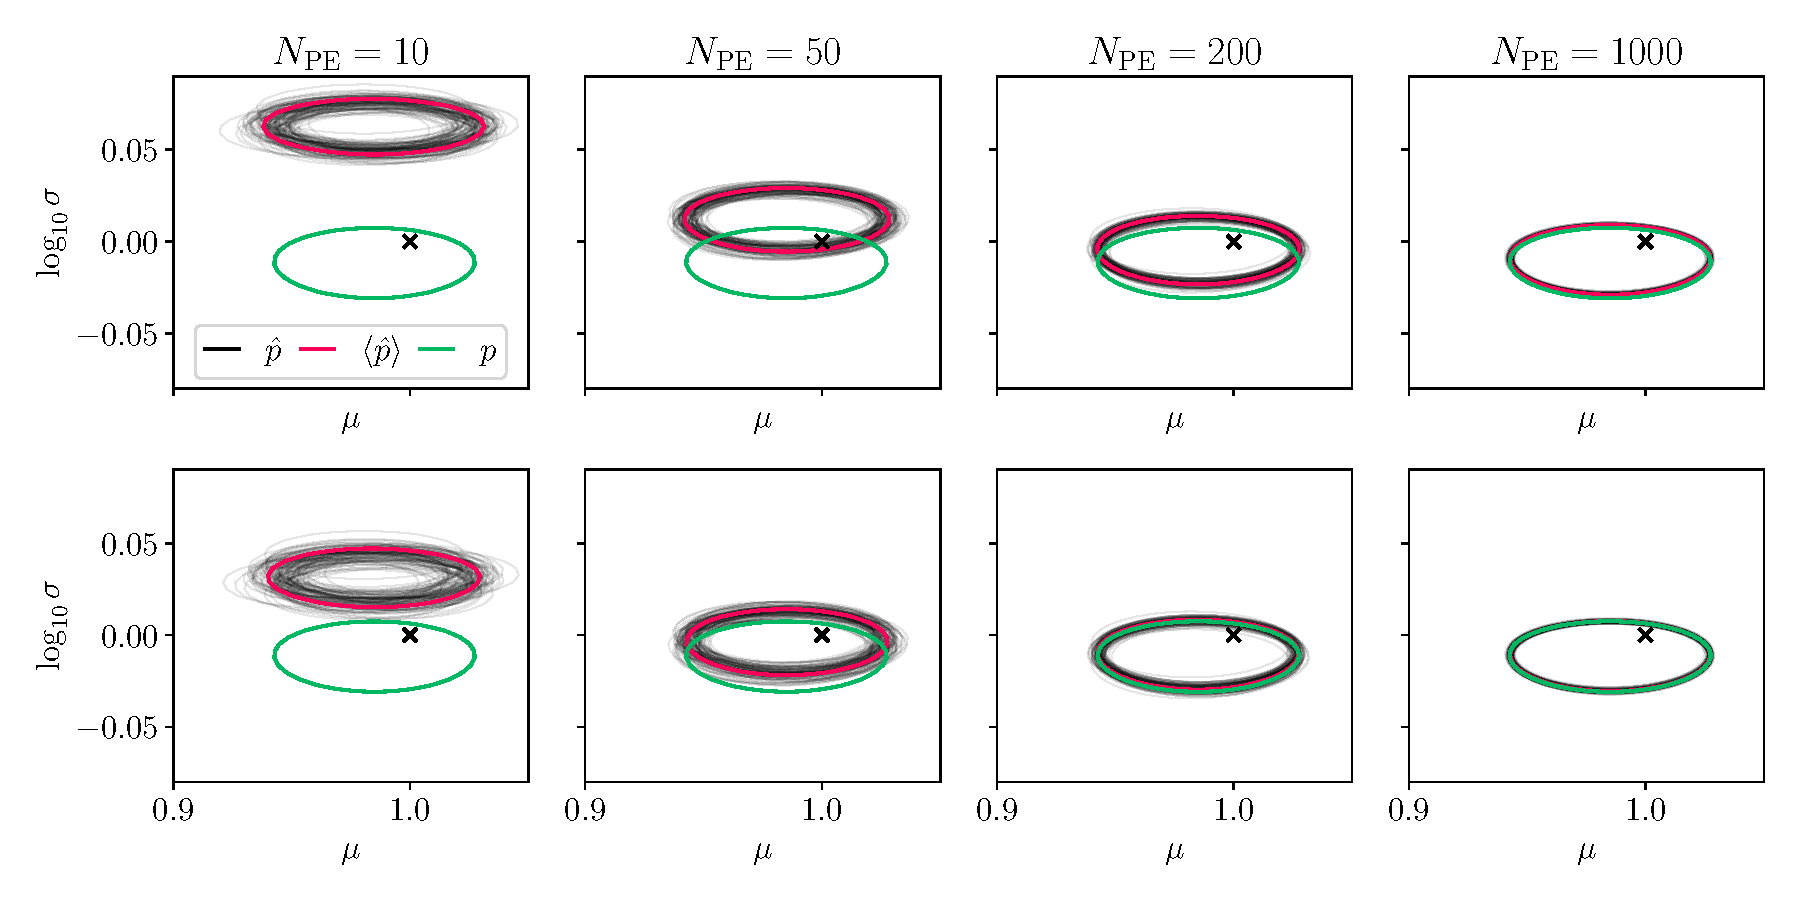
\includegraphics[width=\linewidth]{plots/gaus_hierarchical/pe_uncertainty_only/posteriorComparisons_N5000_4pes.pdf}
    \caption{A comparison between the posterior estimator where $\Nobs=5000$ without correction (in the upper panels) and with correction (in the lower panels). Each black curve represents a 90\% \ac{HPD} contour for an independent posterior estimator, and the red curve represents the mean of the posterior estimators. The green curve is the true posterior computed analytically, and the black $\times$ symbol represents the true hyperparameters $\mu = 1$ and $\sigma = 1$.}
    \label{fig: posterior comparisons nobs 5000}
\end{figure}

\begin{figure}[h!]
    \centering
    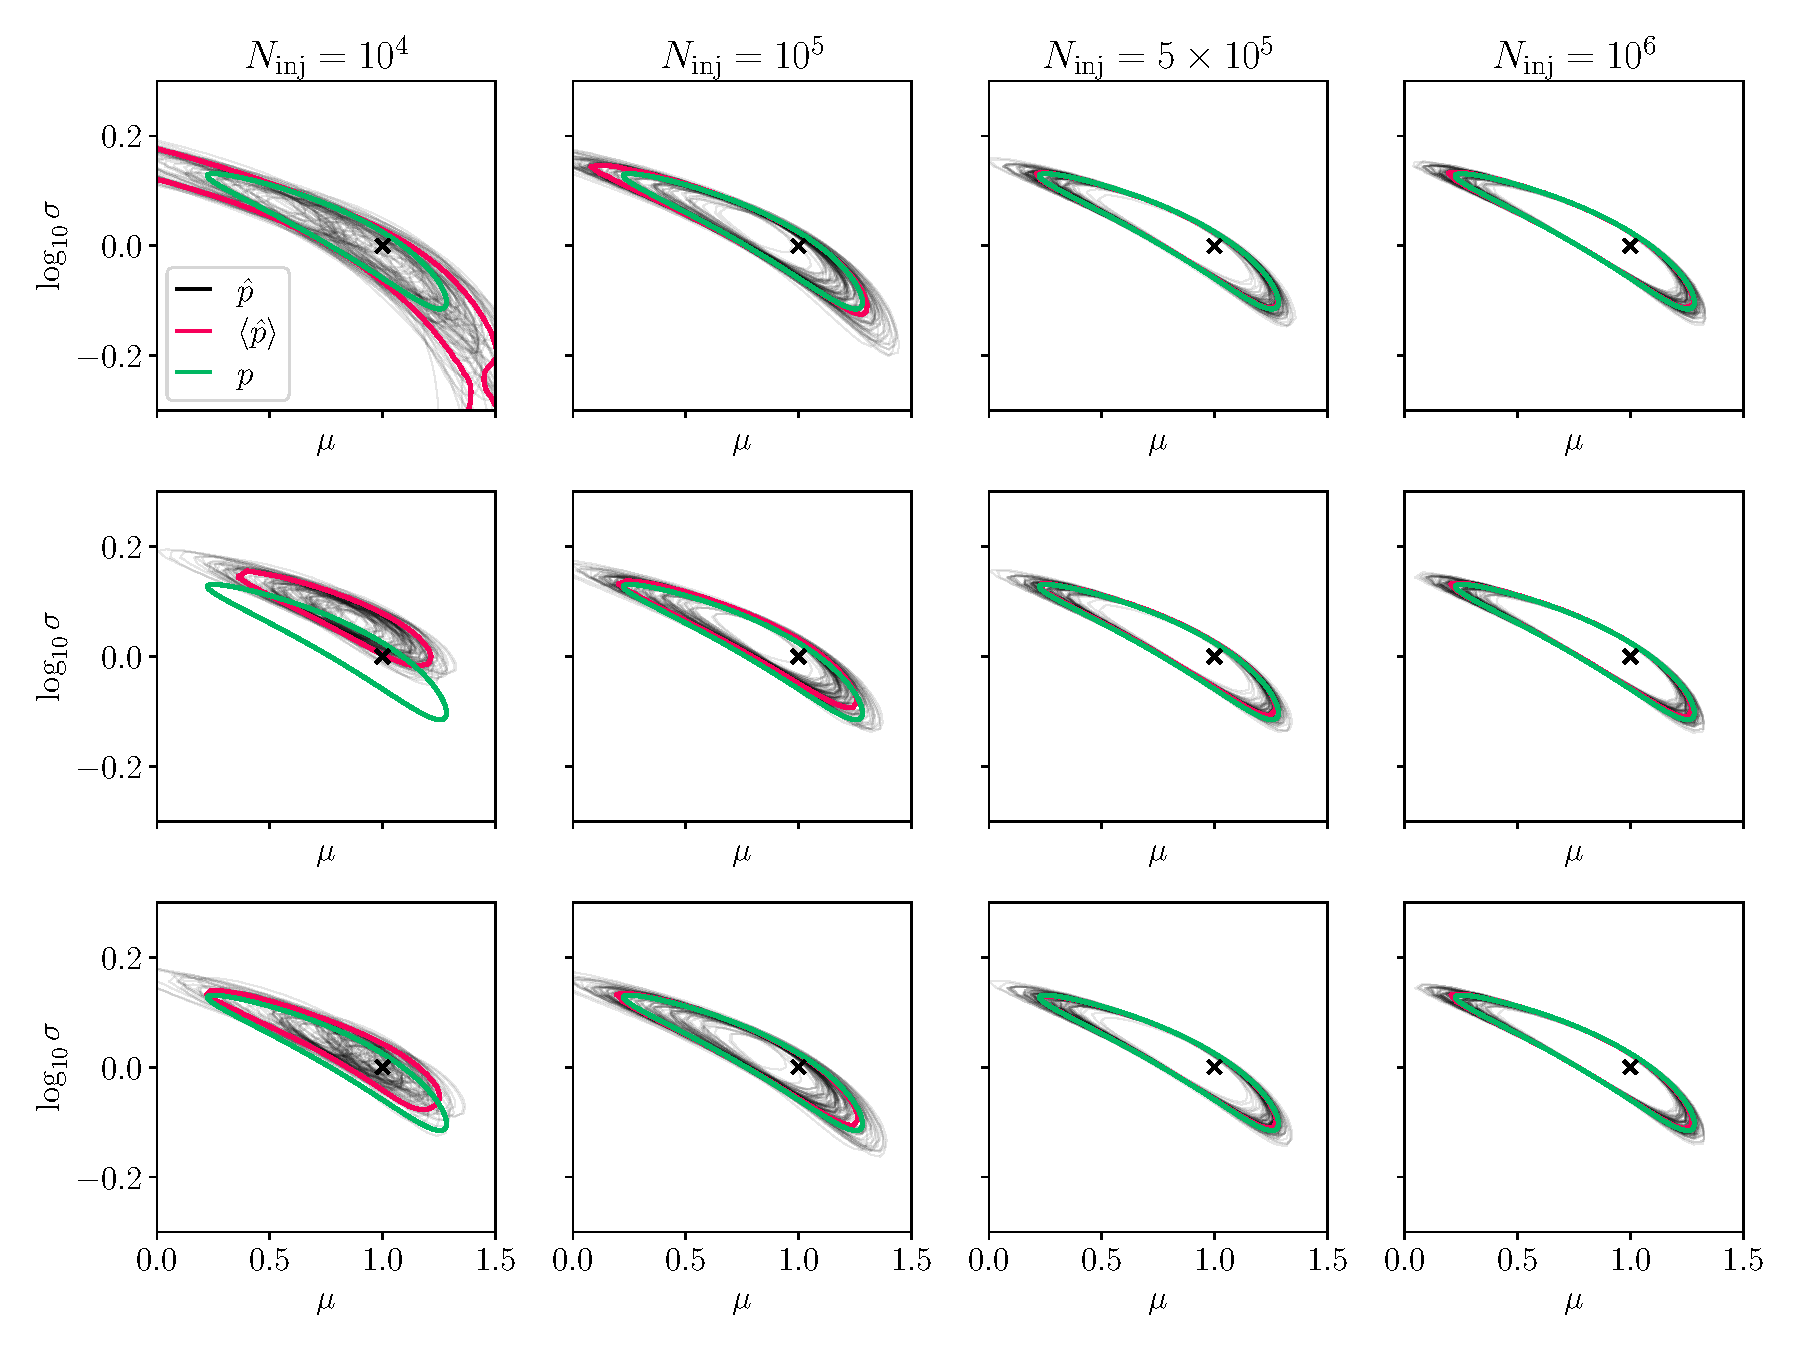
\includegraphics[width=\linewidth]{plots/gaus_hierarchical/selection_effects/posteriorComparisons_selection_1_N1000_4vts.pdf}
    \caption{A comparison between the posterior estimator where $\Nobs=1000$ without any correction (in the top panels), with likelihood correction (in the central panels) and with both likelihood and posterior correction (in the bottom panels). Each black curve represents a 90\% \ac{HPD} contour for an independent posterior estimator, and the red curve represents the mean of the posterior estimators. The green curve is the true posterior computed analytically, and the black $\times$ symbol represents the true hyperparameters $\mu = 1$ and $\sigma = 1$. Here, selection is given by $d = \theta + n>1$.}
    \label{fig: selection posterior comparisons nobs 1000}
\end{figure}


\begin{figure}[h!]
    \centering
    
\includegraphics[width=0.6\linewidth]{plots/larger_KL_npe_noise1.pdf}
    \caption{Empirically measured \ac{KL} divergence from true posterior $p$ and the mean of the posterior estimator $\expect{p}$. We use the same scheme as Fig.~\ref{fig: random KL fn of npe}, using $10^4$ posterior estimators for $\NPE < 90$ and $10^5$ to reduce uncertainty for $\NPE > 90$. We overlay $\NPE^{-2}$ and $\NPE^{-4}$ scaling to show that the posterior correction term removes the leading order posterior bias.}
    \label{fig: random KL fn of npe vs correction}
\end{figure}

Next, we verify that the correction indeed removes the leading order bias. In Fig.~\ref{fig: random KL fn of npe vs correction} we show an analogous figure to Fig.~\ref{fig: random KL fn of npe} where we compute the \ac{KL} divergence from the mean posterior to the true posterior $\KLD(\expect{\hat{p}}|p)$ as a function of $\NPE$ for both the uncorrected and the corrected posterior estimators. With the uncorrected posterior estimator $\hat{p}$, the bias scales as $\NPE^{-1}$ and so the \ac{KL} divergence scales with $\NPE^{-2}$. If the leading order bias in the corrected posterior estimator $\hat{p}_C$ is removed, then the residual bias in should scale with $\NPE^{-2}$ and therefore the \ac{KL} divergence should scale as $\NPE^{-4}$. Figure~\ref{fig: random KL fn of npe vs correction} shows the leading order bias is indeed removed by the correction factor.
